\ifgerman{\chapter{Anhang}}{\chapter{Appendix}}
\label{ch:appedix}
\section{Backpropagation Example}\label{appendix:BackpropExample}

To better understand the backpropagation algorithm mention in \ref{backprop}, consider the following example.

\begin{figure}[!ht]
    \centering
    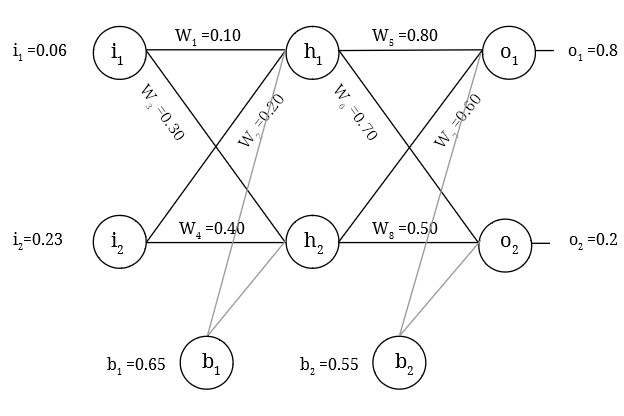
\includegraphics[width=8cm,height=6cm, keepaspectratio]{pics/BackpropExample.jpg}
    \captionsetup{justification=justified,margin=1cm}
    \caption{Basic structure of a neural network with weights and bais initialized}
    \label{fig:bakprop}
\end{figure}

The goal of backpropagation is the adjust the weights such that the neural network can correctly map the input to the output. To begin with consider the neural network in the \ref{fig:bakprop} with inputs to the neural network be $i_{1} = 0.06$ and $i_{2} = 0.23$ to which the neural network should output $o_{1}=0.8$ and $o_{2}=0.2$.

In the forward pass, the neural network is feed in the inputs and given the weights and biases in the \ref{fig:bakprop}, it has to predict the output. It has to figure out the output at each hidden layer neuron, i.e $h_{1}$ and $h_{2}$ and squash each output using activation function and do the same at output layer. The activation function in this case is a \textit{logistic function} of which sigmoid activation is a special case.

To calculate the input at $h_{1}$ as $net_{h_{1}}$ we can use \ref{eq:NNformula} as follows,
\begin{align}
    net_{h_{1}} &= W_{1} * i_{1} + W_{2} * i_{2} +b_{1}\\
    net_{h_{1}} &= 0.10 * 0.60 + 0.20 * 0.23 + 0.65 \\
    net_{h_{1}} &= 0.756 \label{eq:endH1}
\end{align}

And to get the output $out_{h_{1}}$ at $h_{1}$ we apply logistic function to \ref{eq:endH1},
\begin{align}
    out_{h_{1}} &= \frac{1}{1+e^{-net_{h_{1}}}}\\
    out_{h_{1}} &=  \frac{1}{1+e^{0.756}}\\
    out_{h_{1}} &= 0.680 \label{eq:outH1}
\end{align}

Similarly calculating $out_{h_{2}}$ at $h_{2}$ will be:
\begin{align}
    out_{h_{2}} &= 0.681
\end{align}

We can apply same process to output layer neuron, using the output from the hidden layer neuron $h_{1}$ and $h_{1}$ as input.
\begin{align}
    net_{o_{1}} &= W_{5} * h_{1} + W_{7} * h_{2} +b_{2} \label{eq:net_out_1}\\
    net_{o_{1}} &= 0.8 *0.680 +0.6 *0.681 +0.55 \\
    net_{o_{1}} &= 1.50 \label{eq:endO1}
\end{align}
And output $out_{o_{1}}$ at $o_{1}$ we apply logistic function to \ref{eq:endO1}
\begin{align}
    out_{o_{1}} &= \frac{1}{1+e^{-net_{o_{1}}}}\\
    out_{o_{1}} &=  \frac{1}{1+e^{1.50}}\\
    out_{o_{1}} &= 0.8175
\end{align}

Similarly output at $o_{2}$ can be obtained using the same process:
\begin{align}
    out_{o_{2}} &= 0.7957
\end{align}

We have got the output of the final layer, now we can calculate the error. An error function calculates the difference between desired output also known as target and the output predicted by the network. For the purpose of this example we will consider the standard Euclidean distance between the target and the output predicted by the network which we will henceforth refer to as output. 
\begin{align}\label{eq:error}
E_{(target, output)} = \frac{1}{2} (target - output)^{2}    
\end{align}

As we already know the values of the desired output and the predicted output, putting those values in the \ref{eq:error} we can calculate error for $o_{1}$ and $o_{2}$ as follows,

\begin{align}
    E_{o_{1}} &= \frac{1}{2} (0.8-0.8175)^{2}\\
    E_{o_{1}} &= 0.00015  \label{eq:eO1}
\end{align}

Similarly for $E_{o_{2}}$,
\begin{align}\label{eq:eO2}
    E_{o_{2}} &= 0.1774
\end{align}

Combining \ref{eq:eO1} and \ref{eq:eO2} we can calculate total error $E_{total}$ as,
\begin{align}
    E_{total} &= E_{o_{1}} + E_{o_{2}} \label{eq:Etotal}\\
    E_{total} &= 0.17755
\end{align}

Now as the error is calculated we can update the weights so that the predicted outputs are closer to the desired outputs.
Considering the weight $W_{5}$, we want to find out how much change in $W_{5}$ affects the error, i.e the rate of $E_{total}$ w.r.t $W_{5}$, i.e $\frac{\partial E_{total} }{\partial W_{5}}$. 

Applying chain rule, 
\begin{align}
    \frac{\partial E_{total} }{\partial W_{5}} = \frac{\partial E_{total} }{\partial out_{h_{1}}} * \frac{\partial out_{h_{1}} }{\partial net_{h_{1}}} *  \frac{\partial net_{h_{1}} }{\partial W_{5}} \label{eq:backpropMain}
\end{align}

Calculating each term individually,
\begin{align}
    \frac{\partial E_{total} }{\partial out_{h_{1}}} &= \text{change in total loss w.r.t output of $h_{1}$}
\end{align}
From \ref{eq:Etotal}, we can write,
\begin{align}
    E_{total} &= \frac{1}{2}(target_{o_{1}} - out_{o_{1}})^{2} + \frac{1}{2}(target_{o_{2}} - out_{o{1}})^{2}
\end{align}

Taking the partial derivative of $E_{total}$ with respect to $out_{h_{1}}$, the part $\frac{1}{2}(target_{o_{2}} - out_{o{1}})^{2}$ becomes 0 because $out_{h_{1}}$ does not effect it and hence it is a constant.
\begin{align}
    \frac{\partial E_{total}}{\partial out_{o_{1}}} &= 2 * \frac{1}{2}(target_{o_{1}} - out_{o_{1}})^{2 - 1} * -1 + 0\\
    \frac{\partial E_{total}}{\partial out_{o_{1}}} &= -(target_{o_{1}} - out_{o_{1}}) = -(0.8 - 0.8175) = -0.0175 \label{eq:Backprop_2}
\end{align}

Now for the second term in the equation \ref{eq:backpropMain}, we find out the rate of change of $out_{h_{1}}$ w.r.t $net_{h_{1}}$, hence we need to calculate the partial derivative of the logistic function. 
\begin{align}
    out_{h_{1}} &= \frac{1}{1-e^{net_{h_{1}}}}\\
    \frac{\partial out_{h_{1}}}{\partial net_{h_{1}}} &=  out_{h_{1}}*(1-out_{h_{1}}) \\
    \frac{\partial out_{h_{1}}}{\partial net_{h_{1}}} &= 0.8175(1-0.8175) = 0.1491 \label{eq:Backprop_3}
\end{align}
Finally, how much the $n_{o_{1}}$ changes w.r.t $W_{5}$,
\begin{align}
    net_{o_{1}} &= W_{5} * out_{h_{1}} + W_{7} * out_{h_{2}} + b_{2}   \\
    \frac{\partial net_{o_{1}}}{\partial W_{5}} &=  1 * out_{h_{1}} * W_{5}^{(1 - 1)} + 0 + 0 = out_{h_{1}} = 0.680 \label{eq:Backprop_4}
\end{align}

Puttinng \ref{eq:Backprop_2}, \ref{eq:Backprop_3} and \ref{eq:Backprop_4} together, we get:

\begin{align}
    \frac{\partial E_{total} }{\partial W_{5}} &= -0.0175 * 0.1491 * 0.680 = -0.00177429 \label{eq:backprop_6}
\end{align}

To get the new updated weights, we then subtract this the value obtained in \ref{eq:backprop_6} from the old weight multiplying it with learning rate which is 0.1 in our case:

\begin{align}
    W_{5_{new}} = w_5 - \text{learning rate}* \frac{\partial E_{total}}{\partial w_{5}} = 0.8 - 0.1 * (-0.00177429)= 0.800177429
\end{align}

Similarly, we can calculate all the weight updates for $W_{1_{new}}$, $W_{2_{new}}$, $W_{3_{new}}$,$W_{4_{new}}$,\\$W_{6_{new}}$,$W_{7_{new}}$,$W_{8_{new}}$ using the method mentioned above.

\clearpage

\section{Calculating Micro-average Precision Recall and F1-Score}\label{MicroMacroCalculation}
% Please add the following required packages to your document preamble:
% \usepackage{multirow}
% Please add the following required packages to your document preamble:
% \usepackage{multirow}
% Please add the following required packages to your document preamble:
% \usepackage{multirow}

The \ref{tab:precisionRecallF1Score} and \ref{table:Confmatrix1} shows the precision, recall and f1-scores of \gls{BiLSTM} for cluster 1 trained on clustered data show in \ref{fig:question1EvalMacro} and \ref{fig:question1EvalMicro} as BiLSTM-D-ED-C evaluated on document level.

\begin{table}[!ht]
\centering
\begin{tabular}{ccccc}
\textbf{Classes} & \textbf{Precision} & \textbf{Recall} & \textbf{F1-Score} & \textbf{\# Samples} \\ \hline
Agriculture & 0.90 & 0.86 & 0.88 & 50 \\
Audiovisual and Media & 1.00 & 0.10 & 0.18 & 10 \\
Competition & 0.96 & 0.83 & 0.89 & 30 \\
Consumers & 0.59 & 0.65 & 0.62 & 74 \\
Employment and Social Policy & 0.71 & 0.88 & 0.79 & 94 \\
Energy & 0.97 & 0.64 & 0.77 & 56 \\
Enterprise & 0.65 & 0.42 & 0.51 & 26 \\
Environment & 0.70 & 0.84 & 0.76 & 88 \\
Food Safety & 0.93 & 0.82 & 0.87 & 76 \\
Information Society & 0.71 & 0.84 & 0.77 & 80 \\
Internal Market & 0.72 & 0.75 & 0.74 & 148 \\
Public Health & 0.86 & 0.43 & 0.58 & 44 \\
Taxation & 0.95 & 0.71 & 0.82 & 28 \\
Transport & 0.76 & 0.86 & 0.81 & 94 \\ \hline
\textbf{micro avg} & \textbf{0.76} & \textbf{0.76} & \textbf{0.76} & \textbf{898} \\
\textbf{macro avg }& \textbf{0.81} & \textbf{0.69} & \textbf{0.71} & \textbf{898} \\ \hline
\end{tabular}
\captionsetup{justification=centering,margin=1cm}
\caption{CLass-wise precision, recall and f1-score}
\label{tab:precisionRecallF1Score}
\end{table}



\begin{table}[!ht]
\centering
\begin{tabular}{lccccccccccccccccl}
 & \multicolumn{16}{c}{Predicted Values} &  \\
\multicolumn{1}{c}{} &  & \textbf{1} & \textbf{2} & \textbf{3} & \textbf{4} & \textbf{5} & \textbf{6} & \textbf{7} & \textbf{8} & \textbf{9} & \textbf{10} & \textbf{11} & \textbf{12} & \textbf{13} & \textbf{14} & \textbf{} &  \\ \cline{3-16}

\multirow{14}{*}{\rotatebox[origin=c]{90}{Actual Value}} 

& \multicolumn{1}{c|}{\textbf{1}} & \multicolumn{1}{c|}{\hlc[petrol]{43}} & \multicolumn{1}{c|}{0} & \multicolumn{1}{c|}{0} & \multicolumn{1}{c|}{\hlc[yellow]{1}} & \multicolumn{1}{c|}{\hlc[yellow]{2}} & \multicolumn{1}{c|}{0} & \multicolumn{1}{c|}{0} & \multicolumn{1}{c|}{\hlc[yellow]{2}} & \multicolumn{1}{c|}{\hlc[yellow]{2}} & \multicolumn{1}{c|}{0} & \multicolumn{1}{c|}{0} & \multicolumn{1}{c|}{0} & \multicolumn{1}{c|}{0} & \multicolumn{1}{c|}{0} & 50 & \multirow{14}{*}{\rotatebox[origin=c]{270}{Total Samples}} \\ \cline{3-16}

 & \multicolumn{1}{c|}{\textbf{2}} & \multicolumn{1}{c|}{0} & \multicolumn{1}{c|}{1} & \multicolumn{1}{c|}{1} & \multicolumn{1}{c|}{0} & \multicolumn{1}{c|}{0} & \multicolumn{1}{c|}{0} & \multicolumn{1}{c|}{0} & \multicolumn{1}{c|}{0} & \multicolumn{1}{c|}{0} & \multicolumn{1}{c|}{8} & \multicolumn{1}{c|}{0} & \multicolumn{1}{c|}{0} & \multicolumn{1}{c|}{0} & \multicolumn{1}{c|}{0} & 10 &  \\ \cline{3-16}
 
 & \multicolumn{1}{c|}{\textbf{3}} & \multicolumn{1}{c|}{0} & \multicolumn{1}{c|}{0} & \multicolumn{1}{c|}{25} & \multicolumn{1}{c|}{0} & \multicolumn{1}{c|}{0} & \multicolumn{1}{c|}{0} & \multicolumn{1}{c|}{0} & \multicolumn{1}{c|}{0} & \multicolumn{1}{c|}{0} & \multicolumn{1}{c|}{0} & \multicolumn{1}{c|}{1} & \multicolumn{1}{c|}{0} & \multicolumn{1}{c|}{0} & \multicolumn{1}{c|}{4} & 30 &  \\ \cline{3-16}
 
 & \multicolumn{1}{c|}{\textbf{4}} & \multicolumn{1}{c|}{\hlc[red]{2}} & \multicolumn{1}{c|}{0} & \multicolumn{1}{c|}{0} & \multicolumn{1}{c|}{48} & \multicolumn{1}{c|}{1} & \multicolumn{1}{c|}{0} & \multicolumn{1}{c|}{0} & \multicolumn{1}{c|}{2} & \multicolumn{1}{c|}{2} & \multicolumn{1}{c|}{2} & \multicolumn{1}{c|}{11} & \multicolumn{1}{c|}{0} & \multicolumn{1}{c|}{0} & \multicolumn{1}{c|}{6} & 74 &  \\ \cline{3-16}
 
 & \multicolumn{1}{c|}{\textbf{5}} & \multicolumn{1}{c|}{0} & \multicolumn{1}{c|}{0} & \multicolumn{1}{c|}{0} & \multicolumn{1}{c|}{0} & \multicolumn{1}{c|}{83} & \multicolumn{1}{c|}{0} & \multicolumn{1}{c|}{1} & \multicolumn{1}{c|}{0} & \multicolumn{1}{c|}{0} & \multicolumn{1}{c|}{3} & \multicolumn{1}{c|}{7} & \multicolumn{1}{c|}{0} & \multicolumn{1}{c|}{0} & \multicolumn{1}{c|}{0} & 94 &  \\ \cline{3-16}
 
 & \multicolumn{1}{c|}{\textbf{6}} & \multicolumn{1}{c|}{0} & \multicolumn{1}{c|}{0} & \multicolumn{1}{c|}{0} & \multicolumn{1}{c|}{1} & \multicolumn{1}{c|}{0} & \multicolumn{1}{c|}{36} & \multicolumn{1}{c|}{0} & \multicolumn{1}{c|}{14} & \multicolumn{1}{c|}{0} & \multicolumn{1}{c|}{1} & \multicolumn{1}{c|}{2} & \multicolumn{1}{c|}{2} & \multicolumn{1}{c|}{0} & \multicolumn{1}{c|}{0} & 56 &  \\ \cline{3-16}
 
 & \multicolumn{1}{c|}{\textbf{7}} & \multicolumn{1}{c|}{\hlc[red]{3}} & \multicolumn{1}{c|}{0} & \multicolumn{1}{c|}{0} & \multicolumn{1}{c|}{0} & \multicolumn{1}{c|}{3} & \multicolumn{1}{c|}{0} & \multicolumn{1}{c|}{11} & \multicolumn{1}{c|}{2} & \multicolumn{1}{c|}{0} & \multicolumn{1}{c|}{3} & \multicolumn{1}{c|}{4} & \multicolumn{1}{c|}{0} & \multicolumn{1}{c|}{0} & \multicolumn{1}{c|}{0} & 26 &  \\ \cline{3-16}
 
 & \multicolumn{1}{c|}{\textbf{8}} & \multicolumn{1}{c|}{0} & \multicolumn{1}{c|}{0} & \multicolumn{1}{c|}{0} & \multicolumn{1}{c|}{6} & \multicolumn{1}{c|}{2} & \multicolumn{1}{c|}{0} & \multicolumn{1}{c|}{0} & \multicolumn{1}{c|}{74} & \multicolumn{1}{c|}{0} & \multicolumn{1}{c|}{0} & \multicolumn{1}{c|}{2} & \multicolumn{1}{c|}{0} & \multicolumn{1}{c|}{0} & \multicolumn{1}{c|}{4} & 88 &  \\ \cline{3-16}
 & \multicolumn{1}{c|}{\textbf{9}} & \multicolumn{1}{c|}{0} & \multicolumn{1}{c|}{0} & \multicolumn{1}{c|}{0} & \multicolumn{1}{c|}{6} & \multicolumn{1}{c|}{0} & \multicolumn{1}{c|}{0} & \multicolumn{1}{c|}{0} & \multicolumn{1}{c|}{4} & \multicolumn{1}{c|}{62} & \multicolumn{1}{c|}{0} & \multicolumn{1}{c|}{4} & \multicolumn{1}{c|}{0} & \multicolumn{1}{c|}{0} & \multicolumn{1}{c|}{0} & 76 &  \\ \cline{3-16}
 & \multicolumn{1}{c|}{\textbf{10}} & \multicolumn{1}{c|}{0} & \multicolumn{1}{c|}{0} & \multicolumn{1}{c|}{0} & \multicolumn{1}{c|}{0} & \multicolumn{1}{c|}{2} & \multicolumn{1}{c|}{0} & \multicolumn{1}{c|}{0} & \multicolumn{1}{c|}{0} & \multicolumn{1}{c|}{0} & \multicolumn{1}{c|}{67} & \multicolumn{1}{c|}{7} & \multicolumn{1}{c|}{0} & \multicolumn{1}{c|}{0} & \multicolumn{1}{c|}{4} & 80 &  \\ \cline{3-16}
 & \multicolumn{1}{c|}{\textbf{11}} & \multicolumn{1}{c|}{0} & \multicolumn{1}{c|}{0} & \multicolumn{1}{c|}{0} & \multicolumn{1}{c|}{12} & \multicolumn{1}{c|}{7} & \multicolumn{1}{c|}{1} & \multicolumn{1}{c|}{4} & \multicolumn{1}{c|}{1} & \multicolumn{1}{c|}{0} & \multicolumn{1}{c|}{4} & \multicolumn{1}{c|}{111} & \multicolumn{1}{c|}{1} & \multicolumn{1}{c|}{1} & \multicolumn{1}{c|}{6} & 148 &  \\ \cline{3-16}
 & \multicolumn{1}{c|}{\textbf{12}} & \multicolumn{1}{c|}{0} & \multicolumn{1}{c|}{0} & \multicolumn{1}{c|}{0} & \multicolumn{1}{c|}{7} & \multicolumn{1}{c|}{15} & \multicolumn{1}{c|}{0} & \multicolumn{1}{c|}{0} & \multicolumn{1}{c|}{0} & \multicolumn{1}{c|}{1} & \multicolumn{1}{c|}{0} & \multicolumn{1}{c|}{2} & \multicolumn{1}{c|}{19} & \multicolumn{1}{c|}{0} & \multicolumn{1}{c|}{0} & 44 &  \\ \cline{3-16}
 & \multicolumn{1}{c|}{\textbf{13}} & \multicolumn{1}{c|}{0} & \multicolumn{1}{c|}{0} & \multicolumn{1}{c|}{0} & \multicolumn{1}{c|}{0} & \multicolumn{1}{c|}{2} & \multicolumn{1}{c|}{0} & \multicolumn{1}{c|}{0} & \multicolumn{1}{c|}{1} & \multicolumn{1}{c|}{0} & \multicolumn{1}{c|}{2} & \multicolumn{1}{c|}{1} & \multicolumn{1}{c|}{0} & \multicolumn{1}{c|}{20} & \multicolumn{1}{c|}{2} & 28 &  \\ \cline{3-16}
 & \multicolumn{1}{c|}{\textbf{14}} & \multicolumn{1}{c|}{0} & \multicolumn{1}{c|}{0} & \multicolumn{1}{c|}{0} & \multicolumn{1}{c|}{0} & \multicolumn{1}{c|}{0} & \multicolumn{1}{c|}{0} & \multicolumn{1}{c|}{1} & \multicolumn{1}{c|}{6} & \multicolumn{1}{c|}{0} & \multicolumn{1}{c|}{4} & \multicolumn{1}{c|}{2} & \multicolumn{1}{c|}{0} & \multicolumn{1}{c|}{0} & \multicolumn{1}{c|}{81} & 94 &  \\ \cline{3-16}
\end{tabular}
\captionsetup{justification=centering,margin=1cm}
\caption{Confusion matrix for cluster 1 of \gls{BiLSTM} trained on English and German corpus}
\label{table:Confmatrix1}
\end{table}


To calculate the micro average precision we first need the values of \gls{TP} and \gls{FP}. These values are available in confusion matrix in \ref{table:Confmatrix1}

As descibed in \ref{backgroundEvaluationMatrices}, we calculate micro-average precision for a classifier by adding values of $\frac{TP}{TP+FP}$ for all the classes.

Hence, for \textit{Agriculture} the value in the \ref{table:Confmatrix1} for \gls{TP} is highlighted in \hlc[petrol]{blue} and \gls{FP} are highlighted in \hlc[red]{red} and \gls{FN} are highlighted in \hlc[yellow]{yellow}.

 \begin{align}
    \text{Micro-Avg Precision for \textit{Agriculture}} = \frac{43}{43+2+3} 
\end{align}

 \begin{align}
    \text{Micro-Avg Recall for \textit{Agriculture}} = \frac{43}{43+1+2+2+2} 
\end{align}
 
 
Similarly, getting the values of all the classes from the \ref{table:Confmatrix1} we get,

\begin{align*}
    \text{Micro-Avg Precision} =& \frac{43+1+25+48+83}{43+2+3+1+0+25+1+48+33+83+34} \\
    & + \frac{36+11+74+62+67+111}{11+6+74+32+62+5+67+27+111+43}\\
    & + \frac{19+20+81}{19+3+20+1+81+26}
\end{align*}

\begin{align}
    \text{Micro-Avg Precision} = \frac{618}{898} = 0.7583 \approx 0.76
\end{align}

Similarly, to calculate the micro-average recall we get all the \gls{TP} and \gls{TN} values from the confusion matrix,
\begin{align*}
    \text{Micro-Avg Precision} =& \frac{43+1+25}{43+1+2+2+2+8+1+1+25+1+4} \\
    & + \frac{48+83}{48+2+1+2+2+2+11+6+83+1+3+7}\\
    & + \frac{36+11}{36+1+14+1+2+2+11+3+3+2+3+4}\\
    & + \frac{74+62+67}{74+6+2+2+4+62+6+4+4+67+2+7+4}\\
    & + \frac{111}{111+12+7+1+4+1+4+1+1+6}\\
    & + \frac{19+20}{19+7+15+1+2+20+2+1+2+1+2}\\
    & + \frac{81}{81+1+6+4+2}
\end{align*}

\begin{align}
    \text{Micro-Avg Recall} = \frac{618}{898} = 0.7583 \approx 0.76
\end{align}


\begin{align}
    \text{Micro-Avg F1-Score} = &2 * \left ( \frac{\text{micro-avg precision} * \text{micro-avg recall}}{\text{micro-avg precision}+\text{micro-avg recall}} \right ) \\
                              = &2 * \left ( \frac{0.76*0.76}{0.76+0.76} \right ) \\
                              = & 0.76  
\end{align}


To, calculate macro average precision, we need to add the per-class precision values from \ref{tab:precisionRecallF1Score}

Macro-avg precision is, 
\begin{align*}
    =\frac{\text{\small 0.90+1.00+0.96+0.59+0.71+0.97+0.65+0.70+0.93+0.71+0.72+0.86+0.95+0.76}}{\text{\small 14}}
\end{align*}
\begin{align}
    \text{Macro-Avg Precision} =  \frac{11.41}{14} \approx 0.81
\end{align}

Macro-avg recall is, 
\begin{align*}
    =\frac{\text{\small 0.86+0.10+0.83+0.65+0.88+0.64+0.42+0.84+0.82+0.84+0.75+0.43+0.71+0.86}}{\text{\small 14}}
\end{align*}
\begin{align}
    \text{Macro-Avg Precision} =  \frac{}{14} = 0.68785714 \approx 0.69
\end{align}


\section{Visualization of word embeddings} \label{visualEmb}

The visualization of the ten randomly selected words \textit{industrie, alike, customary, siting, thailand, multidisciplinarity, sites, transaktions, hauskatze, formetanate} is given below.

The first step in visualization is to reduce the dimension, for this we are using t-Distributed Stochastic Neighbor Embedding (t-SNE) dimensionality reduction technique. Reducing the dimension is necessary because these words are in 300 dimensional vector space and it would be impossible to consider all the dimension during visualization.

\begin{figure}[!ht]
    \centering
    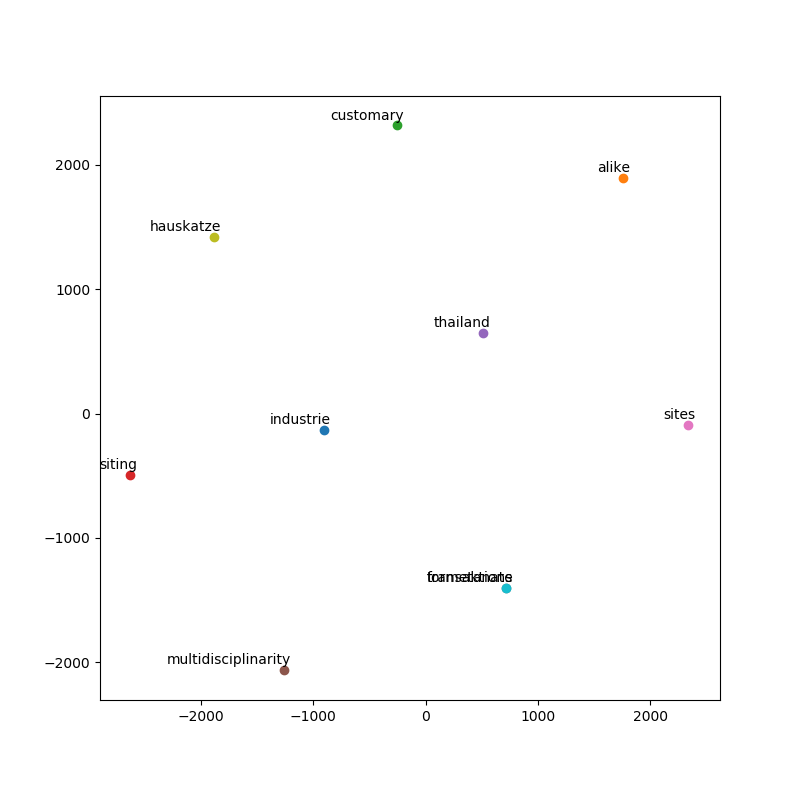
\includegraphics[width=10cm,height=10cm,keepaspectratio]{pics/before_selected_embedding.png}
    \captionsetup{justification=centering,margin=1cm}
    \caption{Visualization of ten randomly selected words for frozen word embedding}
    \label{fig:frozenAppendix}
\end{figure}

As it is clear from the \ref{fig:frozenAppendix} that words like \textit{transaktions} and \textit{formetanate} are not present in the general-purpose embedding and hence their embedding weights are zero and they are coinciding with one another in the \ref{fig:frozenAppendix}.

\begin{figure}[!ht]
    \centering
    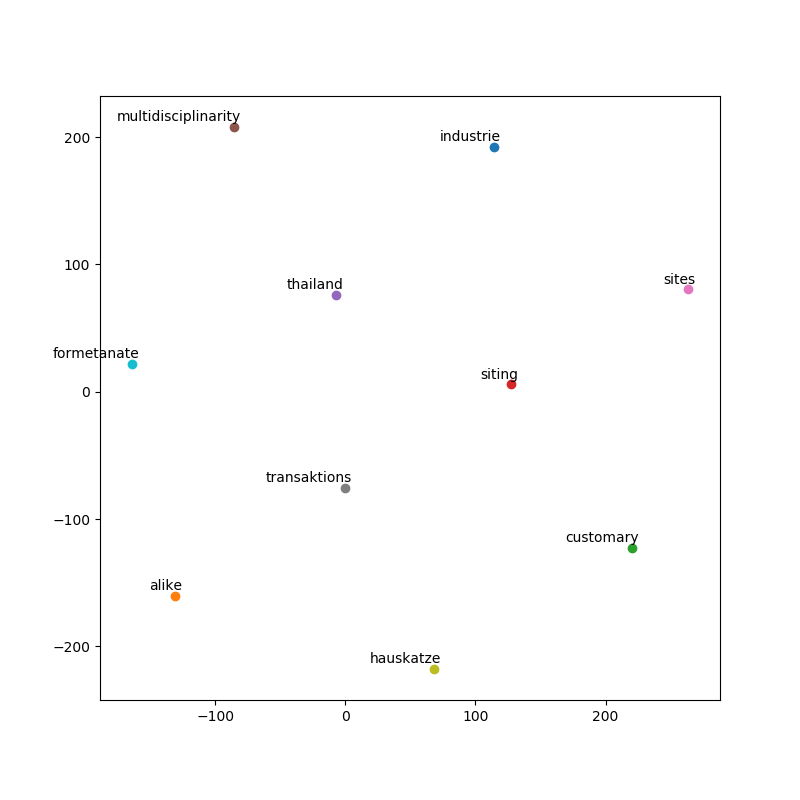
\includegraphics[width=10cm,height=10cm,keepaspectratio]{pics/after_selected_embedding.png}
    \captionsetup{justification=centering,margin=1cm}
    \caption{Visualization of ten randomly selected words for trained word embedding}
    \label{fig:trainedAppendix}
\end{figure}

So we can see that after training \textit{transaktions} and \textit{formetanate} now are at different position \ref{fig:trainedAppendix}. To see the effect of training on these words, we added two new words (\textit{katze},\textit{normal}) and visualized it.

\begin{figure}[!ht]
    \centering
    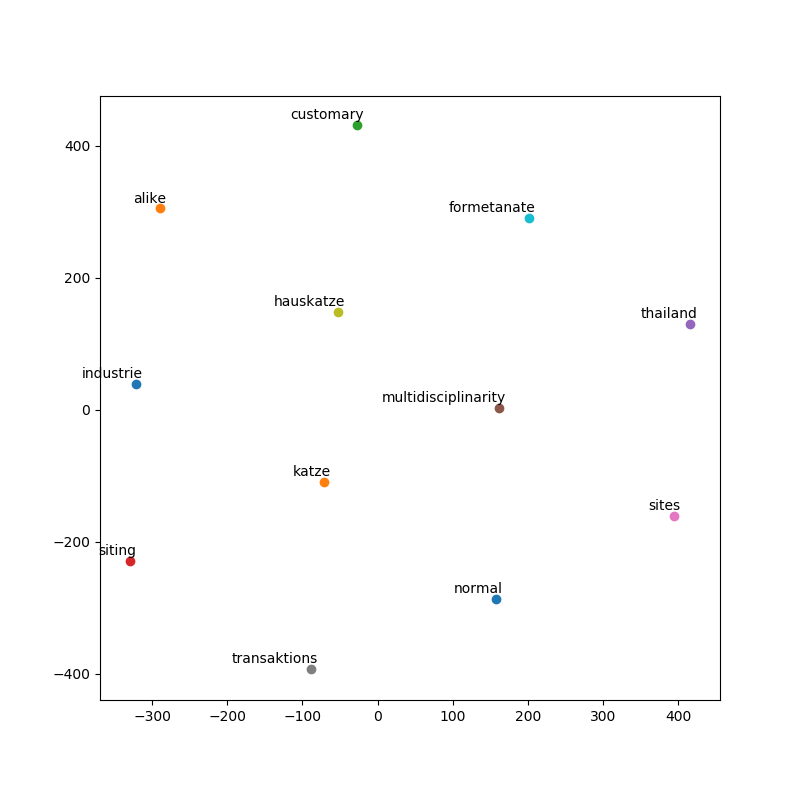
\includegraphics[width=10cm,height=10cm,keepaspectratio]{pics/before_selected_added_embedding.png}
    \captionsetup{justification=centering,margin=1cm}
    \caption{Visualization after adding word \textit{katze} and \textit{normal} to the frozen embeddings}
    \label{fig:frozenAppendixAdded}
\end{figure}

\begin{figure}[!ht]
    \centering
    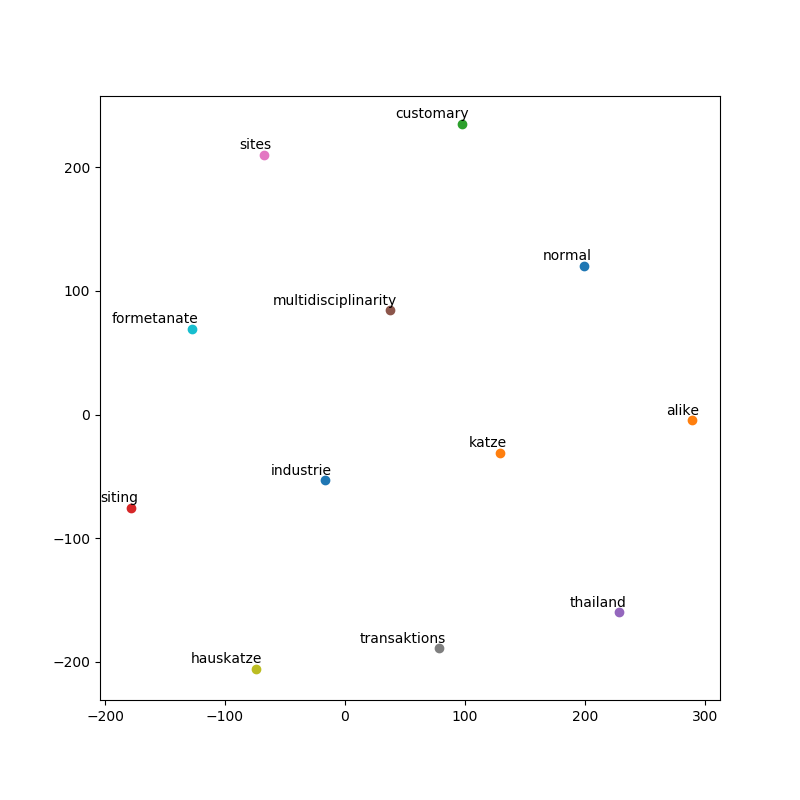
\includegraphics[width=10cm,height=10cm,keepaspectratio]{pics/after_selected_added_embedding.png}
    \captionsetup{justification=centering,margin=1cm}
    \caption{Visualization after adding word \textit{katze} and \textit{normal} to the trained embeddings}
    \label{fig:trainedAppendixAdded}
\end{figure}

\clearpage
The figure \ref{fig:frozenAppendixAdded} shows the added two words before the training of the word embeddings, as we can see that the word \textit{katze} and \textit{hauskatze} are not that far from each other. We can calculate the cosine similarity between these two words before training as follows 
\begin{align}
    \text{cosine similarity before training}_{(katze, hauskatze)} &= \frac{\textbf{katze} \cdot \textbf{hauskatze}}{\left \| \textbf{katze}\right \| \left \| \textbf{hausekatze} \right \|}\\\\
    &= 0.78172445
\end{align}

and the cosine similarity after the embedding is trained is as follows,

\begin{align}
    \text{cosine similarity after training}_{(katze, hauskatze)} = 0.8065112
\end{align}

Similarly, for the words \textit{customary} and \textit{normal} which are synonyms, the cosine similarity before training the embedding and after training embedding 

\begin{align}
    \text{cosine similarity before training}_{(customary, normal)} = 0.18904422
\end{align}

\begin{align}
    \text{cosine similarity after training}_{(katze, hauskatze)} = 0.28809269
\end{align}



Hence, training the embedding further is necessary.